\documentclass[handout, aspectratio=169]{beamer}
\mode<presentation>{}
\usepackage[utf8]{inputenc}
\newcommand{\fl}[1]{\left\lfloor #1 \right\rfloor}

\usepackage{tikz}

\title{MA 105 : Calculus\\ D1 - T5, Tutorial 07}  % change
\author{Aryaman Maithani}
\date[11-09-2019]{11th September, 2019}               % change
\institute[IITB]{IIT Bombay}
\usetheme{Warsaw}
\usecolortheme{beetle}
\newtheorem{defn}{Definition}
\begin{document}
\begin{frame}
	\titlepage
\end{frame}
\begin{frame}{Sheet 5}                            % change
	1. (i)\\
	Writing $y$ in terms of $x$ gives us $y = 1 - 2\sqrt{x} + x.$\\
	The desired area is $$\displaystyle\int_{0}^{1} y dx = \int_{0}^{1} (1 - 2\sqrt{x} + x) dx = \left.\left(x - 2\cdot\frac{2}{3}x^{3/2} + \frac{1}{2}x^2\right)\right|_{0}^{1} = 1 - \frac{4}{3} + \dfrac{1}{2} = \frac{1}{6}. $$\\~\\
	(ii)\\
	Solving for the intersection point of the two curves gives us
	\[x^4 - 2x^2 = 2x^2 \text{ or } x = 0, \pm 2.\]
	It can be verified that for $x \in [-2, 2],$ we have $x^4 - 2x^2 \le 2x^2.$\\
	Thus, the desired area is
	\[\int_{-2}^{2} |x^4 - 2x^2 - 2x^2| dx = \int_{-2}^{2} 4x^2 - x^4 dx = \left.\left(\frac{4}{3}x^3 - \frac{1}{5}x^5\right)\right|_{-2}^{2} = \frac{128}{15}.\]
	
\end{frame}
\begin{frame}{Sheet 5}
	1. (iii)\\
	Solving for the intersection point gives us
	\[3y - y^2 = 3 - y \text{ or } y = 1, 3.\]
	It can be verified that for $y \in [1, 3],$ we have $3y - y^2 \ge 3 - y.$\\
	Thus, the desired area is
	\[\int_{1}^{3} -y^2 + 4y - 3 dy = \left.\left(-\frac{1}{3}y^3 + 2y^2 - 3y\right)\right|_1^3 = \frac{4}{3}. \]
\end{frame}
\begin{frame}{Sheet 5}
	2. It is easy to see that the curves $y = f(x)$ and $y = g(x)$ intersect at $(0, 0)$ and $(1-a, a-a^2).$\\
	Let us assume that $a < 1$ and find the area $A.$
	\[A = \int_{0}^{1-a} (x - x^2 - ax) dx = \frac{(1-a)^3}{6}.\]
	As $A = 4.5,$ we get that $(1 - a)^3 = 27.$ Thus, we have it that $a = -2.$\\
	Now, if we assume that $a > 1,$ we get that $A = \frac{(a-1)^3}{6} = 4.5$ which gives us that $a = 4.$
\end{frame}
\begin{frame}{Sheet 5}
	3. Solving for the intersection point of the two curves gives us
	\[6a\cos\theta = 2a(1+\cos\theta) \text{ or } \theta = \pm\frac{\pi}{3}.\]
	It is for $\theta \in \left(-\dfrac{\pi}{3}, \dfrac{\pi}{3}\right)$ that the circle is outside the cardioid. Thus, the desired area is
	\[A = \frac{1}{2}\int_{-\pi/3}^{\pi/3} (6a\cos\theta)^2 - (2a(1 + \cos\theta))^2 d\theta = 2a^2\int_{-\pi/3}^{\pi/3} 8\cos^2\theta - 1 - 2\cos\theta d\theta\]
	\[= 2a^2\int_{-\pi/3}^{\pi/3} 4\cos(2\theta) - 2\cos\theta + 3 d\theta = 4\pi a^2 \]
\end{frame}
\begin{frame}{Sheet 5}
	6. The region in the $XY$ plane between the two curves is given by $\{(x, y, 0) \in \mathbb{R}^3 : -2 < x < 2, x^2 < y < 8 - x^2\}.$\\
	It can be seen that the plane $y = 4$ is a plane of symmetry for the region. Thus, the centers of the circles mentioned must lie on this plane.\\
	Given a plane $x = x_0,$ the area of the circle of cross-section is given by $\pi(4 - x_0^2)^2.$ Thus, the required volume is
	\[V = \int_{-2}^{2} \pi(4 - x^2)^2 dx = \frac{512\pi}{15}. \]
\end{frame}
\begin{frame}{Sheet 5}
	8. We can fix the line to be along $z-$axis, $0 \le z \le h.$\\
	For any fixed $z,$ the area of the cross-section of the solid is $r^2.$\\
	Thus, the required volume is $\displaystyle\int_{0}^{h} r^2 dz = hr^2.$
\end{frame}
\begin{frame}{Sheet 5}
	9. Washer Method. \\
	In the washer method, the slices are taken \textbf{perpendicular} to the axis of revolution. In this case, the axis of revolution is the line $y = -1.$\\
	Let $f_1(x) := 3 -x^2$ and $f_2(x) := -1$ where both the functions are defined from $[-2, 2]$ to $\mathbb{R}.$ \\
	The volume will given by
	\[V = \pi\int_{-2}^{2} (f_1(x) - (-1))^2 - (f_2(x) - (-1))^2 dx = \pi\int_{-2}^{2} (4 - x^2)^2 dx = \frac{512\pi}{15}. \]
\end{frame}
\begin{frame}{Sheet 5}
	9. Shell Method.\\
	In the shell method, the slivers (which look like cylindrical shells) are taken \textbf{parallel} to the axis of revolution.\\
	For $y_0 \in [-1, 3],$ the line $y = y_0$ cuts the curve at the points $(-\sqrt{3 - y_0}, y_0)$ and $(\sqrt{3 - y_0}, y_0).$ Thus, the height of the sliver is $2\sqrt{3 - y_0}.$\\
	Moreover, the radius, that is, the distance of this sliver from the axis of rotation is: $y_0 + 1.$\\
	Thus, by shell method, we get that the volume of the solid is
	\[V = 2\pi\int_{-1}^{3} (y+1)(2\sqrt{3 - y}) dy = 4\pi\int_{0}^{4} y\sqrt{4 - y} dy = \frac{512\pi}{15}.\]
	The last integral can be calculated easily using Integration by parts.
\end{frame}
\begin{frame}{Sheet 5}
	10. 
	\begin{figure}[h]
		\centering
		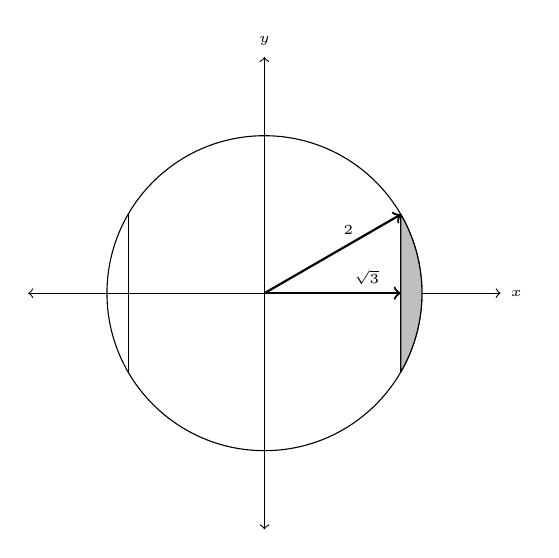
\begin{tikzpicture}
			\def \r{2}
			\def \rt{1.7321}
			\draw[->] (0,0) -- (3,0);
			\draw[->] (0,0) -- (0, 3);
			\draw[->] (0,0) -- (0, -3);
			\draw[->] (0,0) -- (-3,0);
			\draw[thick, ->] (0,0) -- (\rt,0);
			\node[] at (0.75*\rt, 0.2) {\tiny $\sqrt{3}$};

			\draw[thick, ->] (0,0) -- (\rt, 1);
			\node[] at (\rt/2+0.2, 0.5+0.3) {\tiny $2$};

			\node[] at (3.2, 0) {\tiny $x$};
			\node[] at (0, 3.2) {\tiny $y$};
			\draw[] (0, 0) circle (\r);
			\draw[] (\rt, 1) -- (\rt, -1);
			\draw[] (-\rt, 1) -- (-\rt, -1);

			\draw[fill=gray!50] plot[smooth, samples=100, domain=-1:1] %
			({sqrt(4 - (\x*\x))}, {\x}) -| (\rt, -1) -- cycle;
		\end{tikzpicture}
	\end{figure}
\end{frame}
\begin{frame}{Sheet 5}
	10. We can compute the volume of the portion cut out by finding the volume of revolution (about the $y-$axis) of the shaded part. This can be done easily using washer method.\\
	\[V' = \pi\int_{-1}^{1} \left(\sqrt{4 - y^2}\right)^2 - \left(\sqrt{3}\right)^2 dy = \frac{4\pi}{3}. \]
	The total volume of the ball is $V = \dfrac{4\pi}{3}(2)^2.$\\~\\
	Thus, the volume cut out is $V - V' = \dfrac{28\pi}{3}.$
\end{frame}
\end{document}